% !TeX spellcheck = en_US
\documentclass[french]{yLectureNote}

\title{Séries - Analyse 2}
\subtitle{Chimie}
\author{Paulhenry Saux}
\date{\today}
\yLanguage{Français}

\professor{IHallery}%isabelle.hallery@univ-tlse3.fr
\usepackage{graphicx}%----pour mettre des images
\usepackage[utf8]{inputenc}%---encodage
\usepackage{geometry}%---pour modifier les tailles et mettre a4paper
%\usepackage{awesomebox}%---pour les boites d'exercices, de pbq et de croquis ---d\'esactiv\'e pour les TP de PC
\usepackage{tikz}%---pour deiffner + d\'ependance de chemfig
\usepackage{tkz-tab}
\usepackage{chemfig}%---pour deiffner formules chimiques
\usepackage{chemformula}%---pour les formules chimiques en \'equation : \ch{...}
\usepackage{tabularx}%---pour dimensionner automatiquement les tableaux avec variable X
\usepackage{awesomebox}%---Pour les boites info, danger et autres
\usepackage{menukeys}%---Pour deiffner les touches de Calculatrice
\usepackage{fancyhdr}%---pour les en-t\^ete personnalis\'ees
\usepackage{blindtext}%---pour les liens
\usepackage{hyperref}%---pour les liens (\`a mettre en dernier)
\usepackage{caption}%---pour la francisation de la l\'egende table vers Tableau
\usepackage{pifont}
\usepackage{array}%---pour les tableaux
\usepackage{lipsum}
\usepackage{yFlatTable}
\usepackage{multicol}
\newcommand{\Lim}[1]{\lim\limits_{\substack{#1}}\:}
\renewcommand{\vec}{\overrightarrow}
\newcommand{\N}[0]{\mathbb{N}}
\begin{document}
\setcounter{chapter}{0}
\chapter{Électricité }
\section{Mesures en régime continu}
\checkInfo{Tension à vide}{Pour régler la tension à vide, on mesure la tension avec le voltmère directement branché au générateur}
\subsection{Générateur de tension}
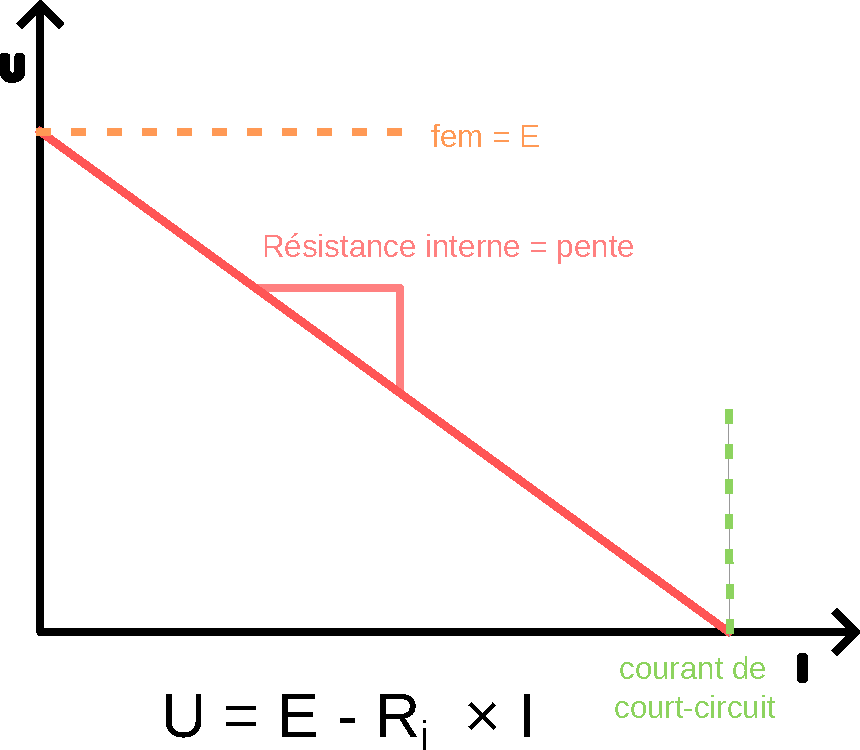
\includegraphics[scale=0.5]{tension}
\begin{definition}
\begin{itemize}
 \item La force électromotrice E du générateur est sa tension à vide, c'est-à-dire la tension entre ses bornes lorsque $I=0$
\item Le courant de court-circuit est le courant quand $U=0$
\item La résistance interne R  est responsable de la chute de la tension que fournit le générateur lorsque l'intensité du courant qu'il délivre augmente.
\end{itemize}

\end{definition}
On réalise le montage suivant, sans oublier la résistance de protection.

En reportant les valeurs, on obtient une fonction constante, ou presque, jusqu'à ce que la fonction diminue subitement.

Dans la plage de courant où la tension est constante, la résistance interne est nulle.

\subsection{Générateur de courant}
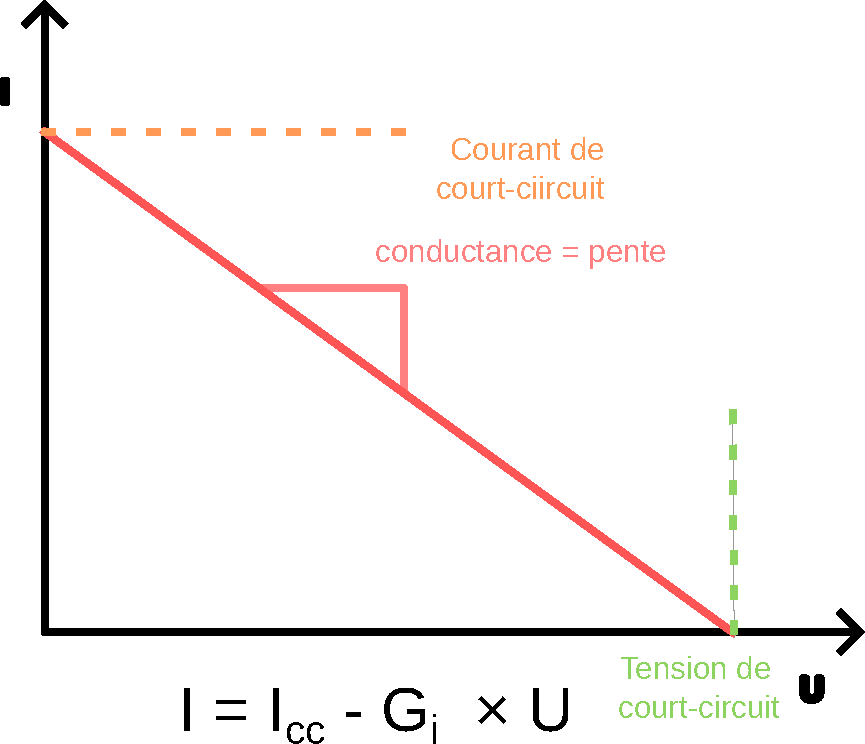
\includegraphics[scale=0.5]{courant}
\tipsInfo{Résistance interne}{
Pour trouver la résistance interne, on calcule la tension aux bornes des résistances placées. On sait aussi la tension que doit délivrer le générateur théoriquement. Expérimentalement, on place un voltmètre et un ampère-mètre pour déterminer le courant et la tension aux borne des résistances placées.

On a donc $E = U + R_i\times I$}
\section{Mesure expérimentale}
On réalise le montage suivant, sans oublier la résistance de protection.

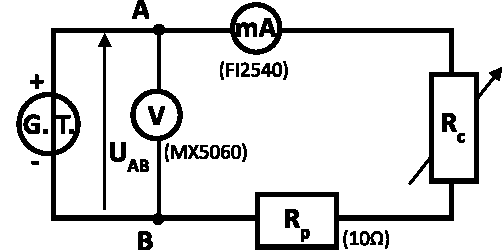
\includegraphics{circuit}

En reportant les valeurs, on obtient une fonction constante, ou presque, pour un générateur idéal ou une fonction affine pour un générateur réel.

\end{document}

